\begin{frame}{Causal state abstractions}
    \begin{itemize}
        \item State abstraction or \enquote{coarse graining} is a key concept in RL.
        \item Any grouping or clustering of states is an \enquote{abstraction}.
        \item How to decide what is a good versus bad grouping?
        \bigskip
        \item \textbf{Key idea}: Causality is useful to measure abstraction quality.
    \end{itemize}

    \mybox{0.7, 0.5}{\fullcite{herlauReinforcementLearningCausal2022}}
\end{frame}

\begin{frame}{State abstractions}
\begin{itemize}
    \item Benefits include:
    \begin{itemize}
        \item More efficient computation and learning.
        \item Facilitate exploration and generalization.
        \item Synergy with composition and communication.
    \end{itemize}
\end{itemize}
    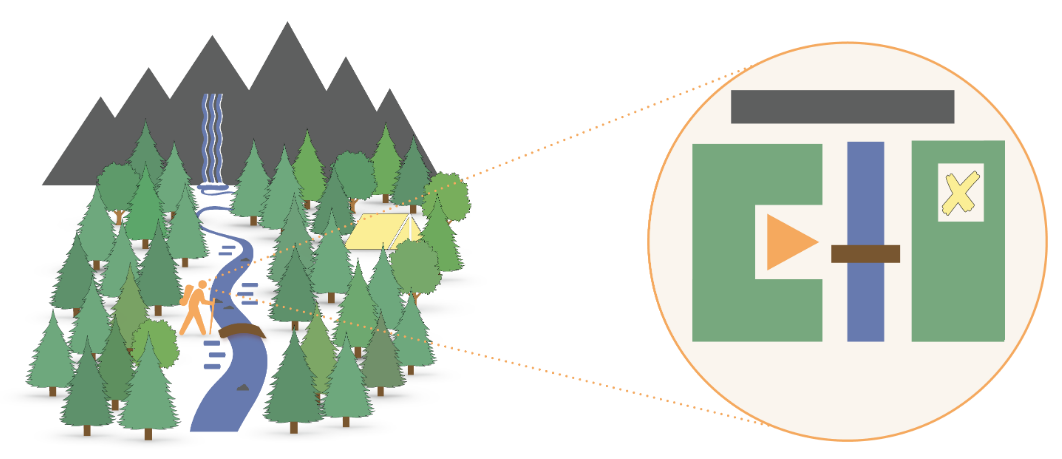
\includegraphics[width=0.58\textwidth]{images/valueofabstraction.png}
    \mybox{0.7, 0.45}{\fullcite{hoValueAbstraction2019}}
\end{frame}


\begin{frame}{Causality?}
    \begin{itemize}
        \item Fundamentally: \enquote{Nature} and the data it generates are intrinsically different.
        \item We model nature by having variables \enquote{listen} to their causes.
        \item Precisely formalized by Pearl and collaborators.
        \bigskip
        \item This implies a \textbf{causal hierarchy} or \textbf{ladder}.
    \end{itemize}
    
    %\begin{textblock}{0.4}(0.7, 0.5)\dbox{
    %\begin{minipage}{\dimexpr\textwidth-2\fboxsep-2\fboxrule\relax}
    %\scriptsize
    %\fullcite{pearlCausality2009a}
    %\end{minipage}}\end{textblock}
    \mybox{0.7, 0.5}{\fullcite{pearlCausality2009a}}
\end{frame}

\note[itemize]{
    \item But first off, what do I mean by causality?
}

\begin{frame}{Ladder of causation: seeing}
    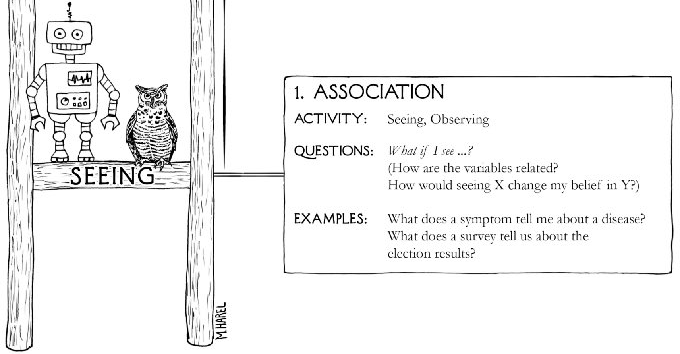
\includegraphics[width=0.9\textwidth]{images/ladder-of-causation-seeing.png}
    \mybox{0.7, 0.5}{\fullcite{pearlBookWhyNew2018}}
\end{frame}

\note{Layer 1 deals with purely “observational”, factual information}

\begin{frame}{Ladder of causation: doing}
    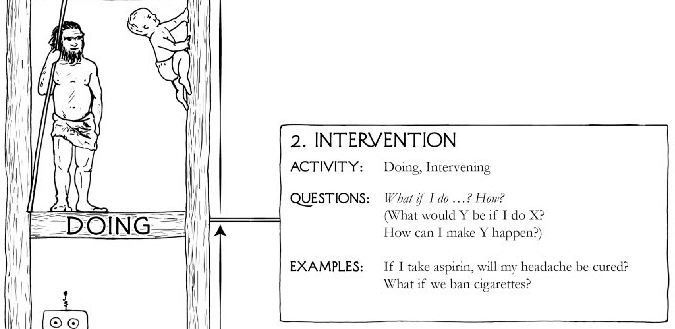
\includegraphics[width=0.9\textwidth]{images/ladder-of-causation-doing.png}
\end{frame}

\note[itemize]{
    \item Rung 2 encodes information about what would happen, hypothetically speaking, were some intervention to be performed, namely effects of actions.
}

\begin{frame}{Ladder of causation: imagining}
    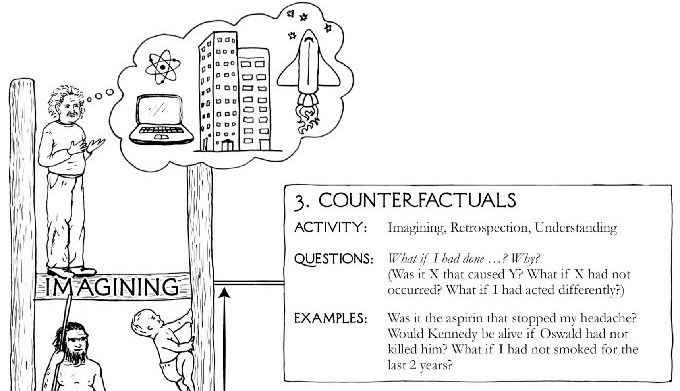
\includegraphics[width=0.88\textwidth]{images/ladder-of-causation-imagining.png}
\end{frame}

\note[itemize]{
    \item Finally, Layer 3 involves queries about what would have happened, counterfactually speaking, had some intervention been performed, given that something else in fact occurred (possibly conflicting with the hypothetical intervention). 
    \item The hierarchy establishes a useful classification of concepts that might be relevant for a given task, thereby also classifying formal frameworks in terms of the questions that they are able to represent, and ideally answer.
}

\begin{frame}{Some intuition on \enquote{causal} models}
    \begin{itemize}
        \item Not a binary concept: degrees of causality.
        \item Rung 2-causality: predictive accuracy of interventional queries.
        \item Rung 3-causality: predictive accuracy of counterfactual queries.
        \bigskip
        \item Humans have (sometimes) reasonably accurate counterfactual models!
    \end{itemize}
\end{frame}

\note[itemize]{
    \item So before moving on: my view
    \item I would not say a model is strictly "causal" or "not causal"
    \item Just like rung 1 associative models can be better or worse
    \item Models are still just models, some are more useful than others
    \item Intuition: Degrees of causality in models
    \item Corresponding to predictive accuracy
    \item Especially counterfactual accuracy can be hard to measure
    \item But humans manage to think and talk about counterfactuals every day
}

\begin{frame}{Structural Causal Models (SCMs)}
    \begin{itemize}
        \item An SCM consists of two sets of variables, $U$ and $V$, a distribution $P(U)$ and a set of mappings,
        \begin{equation*}
            v_i \leftarrow f_i(pa_i, u_i),
        \end{equation*}
        where $pa_i$ are the \emph{parents} of $v_i \in V$.
        \item The variables in $V$ are \emph{endogenous}, and are explicitly considered in the model, i.e. they are on the left hand side of one of the mappings.
        \item The variables in $U$ are \emph{exogenous}, and only appear in the functions $f_i$.
        \item For $Y \subseteq V$ in SCM $M$:
        \begin{equation*}
            P^M(y) = \sum_{\{u | Y(u) = y\}}P(u).
        \end{equation*}
        \item Every SCM is associated with a graph: nodes represent the variables in $U \cup V$, and directed edges represent the functions $f_i$.
    \end{itemize}
\end{frame}

\note[itemize]{
    \item Let's get into some formalities about causal models.
    \item SCMs are how we describe relevant aspects of the world.
    \item In essence, we assume that such an underlying data generating process exists, even though we cannot in general observe this process.
    \item The graph contains less information than the fully specified SCM: only which variables "listen" to others.
}


\begin{frame}{Queries in SCMs}
    \begin{itemize}
        \item For $X \subseteq V$, a \emph{submodel} $M_x$ of an SCM $M$ is
        \begin{equation*}
            M_x = \langle U, V, F_x, P(U) \rangle,
        \end{equation*}
        where
        \begin{equation*}
            F_x = \{f_i : V_i \notin X \} \cup \{X \leftarrow x\}.
        \end{equation*}
        \item The \emph{potential response} defines the rung 2 query,
        \begin{equation*}
            P(Y | do(X = x) = P^{M}(Y_x) = \sum_{\{u | Y_{M_x}(u) = y\}}P(u).
        \end{equation*}
        \item Rung 3 queries are defined, for counterfactual events $Y_x, \dots, Z_w$, as
        \begin{equation*}
            P^M(y_x, \dots, z_w) = \sum_{\{u | Y_{M_x}(u) = y, \dots, Z_{M_w}(u) = z\}}P(u).
        \end{equation*}
    \end{itemize}
\end{frame}

\note[itemize]{
    \item Just for the sake of it, let's quickly go through what it means to answer rung 2 and 3 queries.
    \item Rung 2: 
    \item Rung 3: note that the l.h.s. contain variables with different subscripts. These encode different counterfactual "worlds", and thus no experiment in the world (rung 2) is sufficient to answer the query. 
}

\begin{frame}{The causal agent}
    \includegraphics[width=.9\linewidth]{causal_figures/conceptA}
\end{frame}

\note[itemize]{
    \item This is our imagined setting - an agent possessing a causal model which is an abstraction over the states of the world.
    \item How would an agent go about acquiring a simple causal model of its environment?
    \item We're considering an RL setting, so of course the reward is important - we want to maximize it.
    \item Simultaneously, we want our choice in behavior to be considered with respect to how it affects the outcome.
    
}



\begin{frame}{Mediation analysis}
    \centering
    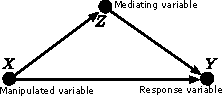
\includegraphics[width=0.4\linewidth]{causal_figures/medanal1}%\hspace{1cm}
    \begin{itemize}
        \item Mediation analysis deals with decompositions of effects into \emph{direct} and \emph{indirect} effects.
        \item The \emph{total} effect is $P(Y_x = y)$, as usually measured in randomized trials.
    \end{itemize}
    %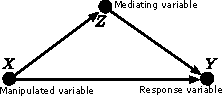
\includegraphics[width=0.4\linewidth]{causal_figures/medanal1}%\hspace{1cm}
    %\includegraphics[width=0.45\linewidth]{causal_figures/medanal2}
    %\begin{align*}
    %	\textrm{NIE} & = \left( \EE\left[Y | Z=1, \pi_a \right] - \EE\left[Y | Z=0, \pi_a \right] \right)  \\  
    %	& \times  \left( P(Z=1| \pi_b) -P(Z=1| \pi_a) \right).
    %\end{align*}
    \mybox{0.70, 0.47}{\fullcite{pearlDirectIndirectEffects2001}}
\end{frame}

\note[itemize]{
    \item ?
}

\begin{frame}{The natural indirect effect}
    \begin{itemize}
        \item An event $X = x$ is said to have an indirect effect on Y (in situation $U = u)$ if
        \begin{equation*}
            \mathrm{NIE}(u) = Y_{x', Z_x(u)}(u) \noteq Y_{x'}(u).
        \end{equation*}
        \item We can thus define the average indirect effect in general as
        \begin{equation*}
            \mathrm{NIE} = \E_u[Y_{x', Z_x(u)}(u)] - \E_u[Y_{x'}].
        \end{equation*}
        \item This is a \emph{nested} counterfactual and can only be identified in specific cases.
    \end{itemize}
\end{frame}

\note[itemize]{
    \item Now let's talk about the specific causal analysis that we use.
    \item The natural indirect effect, or just the indirect effect (since there is no controlled equivalent as in the direct effect), is:
    \item The value of Y changes when we keep X fixed at a reference $X = X'$ while changing Z to the value $Z_x$ that it would attain under $x$.
}

\begin{frame}{Identifying the NIE}
    \centering
    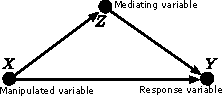
\includegraphics[width=0.5\linewidth]{causal_figures/medanal1}%\hspace{1cm}
    \begin{itemize}
        \item In this simple graph, the NIE is identified even without performing any experiments:
        \begin{equation*}
            \mathrm{NIE} = \sum_z\E[Y | x', z][P(z|x) - P(x | x')].
        \end{equation*}
    \end{itemize}
\end{frame}

\note[itemize]{
    \item This is under the condition that there exists a set $W$ of non-descendants of $X$ or $Z$ s.t. $Y_{x'z} \indep Z_x | W$.
}

\begin{frame}{Assigning variables}
    \centering
    \includegraphics[width=0.5\linewidth]{causal_figures/medanal2}
    
    \begin{itemize}
        \item With binary variables, the NIE further simplifies,
        \begin{align*}
        	\mathrm{NIE} & = \left( \E\left[Y | Z=1, \pi_a \right] - \E\left[Y | Z=0, \pi_a \right] \right)  \\  
        	& \times  \left( P(Z=1| \pi_b) -P(Z=1| \pi_a) \right).%\label{eq12}
        \end{align*}
    \end{itemize}

\end{frame}

\note[itemize]{
    \item Now we specify the meaning of variables in our simple mediation graph.
    \item Choosing binary variables further simplifies the NIE as well.
    \item In this form, we can easily understand what a high value of the NIE means:
    \item The first term relates to the reward outcome Y, and specifies that the causal state Z should be associated with a higher reward.
    \item The second term relates to the agents choice of policy, and specifies that the causal state should be more achievable with policy B. 
    \item As we'll see, policy A going to be a prespecified policy. 
}

\begin{frame}{Implementation: $Z$}
    \begin{itemize}
        \item We model $Z$ as a kind of \emph{stopped process}:
        \begin{equation*}
        	Z = \max\{Z_0, Z_1, \dots Z_T\}.
        \end{equation*}	
        \item Each $Z_t \in \{0,1\}$ is parameterized by a function approximator $\Phi$:
        \begin{equation*}
            Z_t \sim \textrm{Bern}(\Phi(s_t)).
        \end{equation*}
    \end{itemize}
\end{frame}

\note[itemize]{
    \item 
}

\begin{frame}{Implementation: $\pi$}
	\centering
	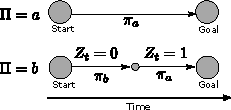
\includegraphics[width=0.4\linewidth]{causal_figures/medanal3}

	\begin{itemize}
    	\item The combined policy will either follow $\pi_a$, or follow the alternative policy $\pi_b$ until $Z$ is true after which it follows $\pi_a$. 
    \begin{align*}
    	\pi = \begin{cases} \pi_a & \mbox{if $\Pi = a$ } \\ \left(1-\max\{Z_{0}, \dots, Z_t\} \right)\pi_b +\max\{Z_{0}, \dots, Z_t\} \pi_a
    		& \mbox{if $\Pi = b$. }\end{cases} %\label{eq10}
    \end{align*}
	\end{itemize}	
\end{frame}

\note[itemize]{
    \item We implement the policy choice in a specific way.
    \item This is motivated by the term in the NIE that encourages $pi_b$ to reach $Z=1$.
    \item Additionally, the interpretation of $pi_b$ as part of a hierarchical policy is interesting.
}

\begin{frame}{Implementation: Maximization}
    \begin{itemize}
    	\item How to maximize the NIE wrt. $Z$ and $\pi_b$?
    	\begin{align*}
    		\mathrm{NIE} & = \left( \E\left[Y | Z=1, \pi_a \right] - \E\left[Y | Z=0, \pi_a \right] \right)  \\  
    		& \times  \left( P(Z=1| \pi_b) -P(Z=1| \pi_a) \right).%\label{eq12}
    	\end{align*}
    \item Estimate this quantity iteratively, in the same way as the Bellman iteration for the value function,
    \begin{equation*}
        V(s_{t} ) = \E[ R_{t+1} + \gamma V(s_{t+1}) | S_t=s_t].
    \end{equation*}

    \end{itemize}
\end{frame}

\note[itemize]{
    \item asd
}

\begin{frame}{Z-value functions}
We define the set of variables
\begin{equation*}
	Z_t^\infty = \max\{Z_t,Z_{t+1}, \dots,\}, %(1-Z_{k-1}) = \mbox{One of $Z_k,\dots$ is true and $Z_k$ is false}
\end{equation*}
each of which is $1$ at time $t$ if $Z$ becomes $1$ at any time $t$ or later -- and $0$ otherwise.
Our goal is then to estimate the quantities
\begin{align*}
	v^{\infty}_t(s_t) & = P(Z^\infty_t =1 | S_t=s_t, Z_{t-1} = 0), \\
	v^{z}_t(s_t) & = \E\left[G_t | S_t=s_t, Z_t^\infty = z, Z_{t-1} = 0\right],  %\label{eq19} 
\end{align*}
both of which are conditional on $Z_{t-1} = 0$.

These quantities satisfy mutually recursive equations which can be jointly estimated with standard algorithms.
%They satisfy recursions
%\begin{subequations} 
%\begin{align*}
%		v^\infty_t(s_t) & = \Phi(s_t) + (1-\Phi(s_t) ) \E\left[ v^\infty_{t+1}(S_{t+1} )| s_t\right],  \\ 
%		v^{1}_t(s_t) & =  \frac{ V(s_t) \Phi(s_t) }{V_t^\infty(s_t) }  
%		+ \frac{  1\!-\! \Phi(s_t)  }{V_t^\infty(s_t) } \E\left[ v^\infty_{t+1}(S_{t+1}) \left( R_{t+1} + \gamma v^{1}_{t+1}(S_{t+1} ) \right) \mid s_t   \right], \nonumber \\	
%\end{align*}
%\end{subequations}
%Both have the form
%\begin{align*}
%	v_t(s_t) & =\E\left[H_t(s_t,S_{t+1})  + G_t(s_t, S_{t+1}) v_{t+1}(S_{t+1} )  )  \middle| s_t\right] %\label{eq22a}
%\end{align*}
\end{frame}

\note[itemize]{
    \item The first denotes the event that $Z=1$ will happen in the future given that it has not yet.
    \item The second is the expected return given that Z has not happened yet, and that it will ($z=1$) or that it won't ($z=0$).
    \item Note that $v^\infty_0(s_0) = P(Z = 1| s_0)$ and $v^z_0(s_0) = \E[G_0 | s_0, Z=z]$.
    \item Luckily, those are also terms in our simplified NIE!
    \item 
}

\begin{frame}{Example: two-stage environment}
\centering
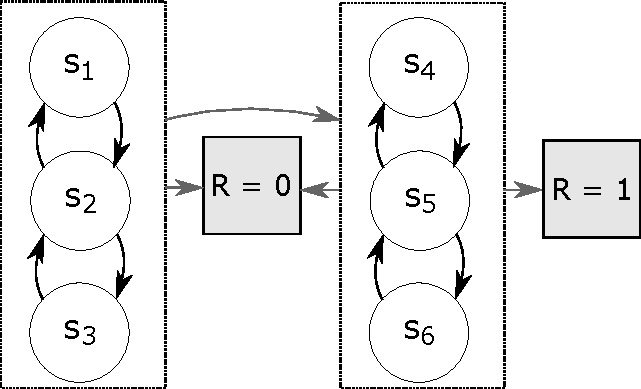
\includegraphics[width=.28\linewidth]{causal_figures/twostage}
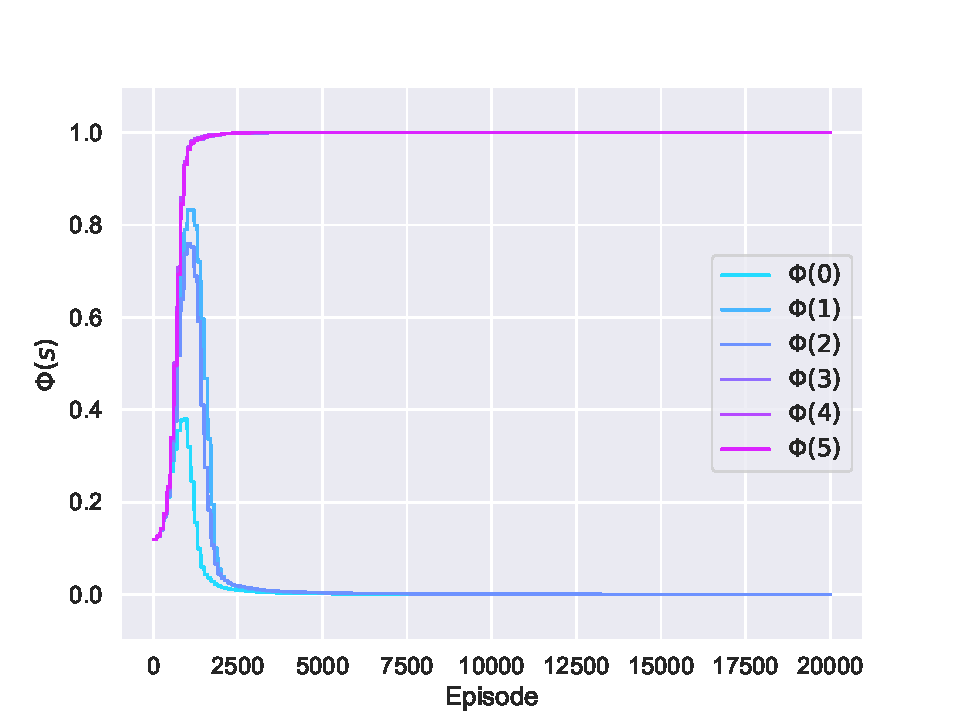
\includegraphics[width=.48\linewidth]{causal_figures/twostage_Phi}~
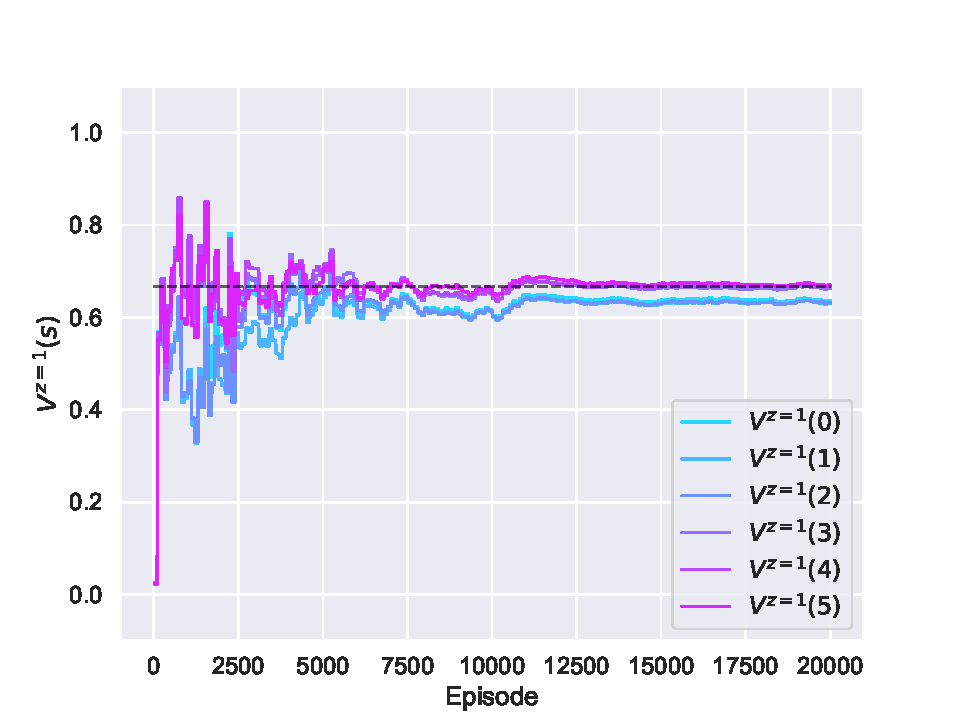
\includegraphics[width=.48\linewidth]{causal_figures/twostage_Vz1}
\end{frame}

\begin{frame}{Example: Doorkey environment}
\centering
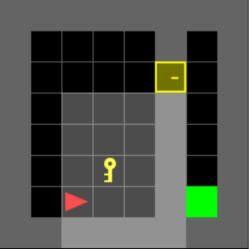
\includegraphics[width=.33\linewidth]{causal_figures/doorkey}~
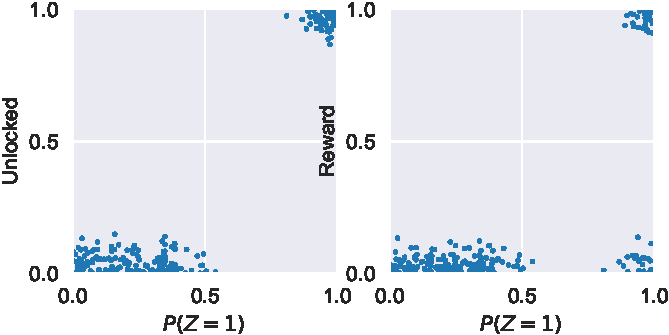
\includegraphics[width=0.66\linewidth]{causal_figures/scatter_AB}
\begin{itemize}
	\item Trained on a small Doorkey environment.
	\item Learned variable $Z$ corresponds to unlocking the door.
\end{itemize}
\end{frame}

\note[itemize]{
    \item Doorkey environment not shown, but pretty simple to explain.
    \item Left: Chance of unlocking door at each P(Z=1).
    \item Right: Chance of reaching goal state at each P(Z=1).
}

\begin{frame}\frametitle{Causality and optimal policies?}
    \begin{align*}
    	\mathrm{NIE} & = \left( \E\left[Y | Z=1, \pi_a \right] - \E\left[Y | Z=0, \pi_a \right] \right)  \\  
    	& \times  \left( P(Z=1| \pi_b) - P(Z=1| \pi_a) \right).%\label{eq12}
    \end{align*}
    \begin{itemize}
    \item The NIE will generally not be large when $\pi_a$ is optimal
    \item How well-defined is the notation of a parsimonious causal model when an optimal policy is known? 
    \end{itemize}
\end{frame}

\begin{frame}{Recent related work and future work}
    \begin{center}
        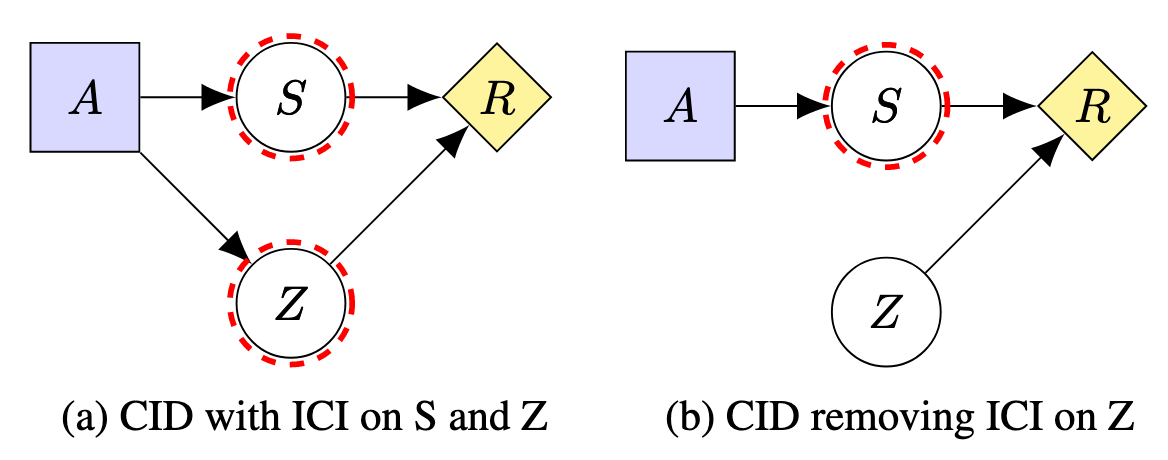
\includegraphics[width=.5\textwidth]{images/cid.png}
    \end{center}
    
    Future work:
    \begin{itemize}
    \item Unifying view of more concepts, e.g. agent safety using causality?
    \item Too heavy assumptions - can we remove some?
    \item Scaling up - sample efficiency and instability.
    \end{itemize}

    \mybox{0.01, 0.225}{\fullcite{farquharPathspecificObjectivesSafer2022}}
\end{frame}

\note[itemize]{
    \item I wanted to point out some related work that was also accepted at AAAI 2022.
    \item Here, Causal Influence Diagrams (as shown) describe a framework for safe training of agents whose \textbf{naive incentives} are unsafe.
    \item ICI = Instrumental Control Incentive, the red circles. Blue square is decision. Yellow diamond is utility. Black arrows show causal influence.
    \item Traditional RL obviously fails: expected return is maximized by any means.
    \item Their method trains agents by essentially optimizing only the \textbf{direct effect}, disallowing indirect effects through unsafe (aka delicate) causal states.
    \item Some future work for our setting:
    \item We use a simple setting in order for the NIE to be identifiable from *observational data* - but we aren't in a strictly observational setting. We can do experiments - which assumptions can we then remove, that we used to identify the NIE?
}




